\chapter{Технологическая часть}
\section{Средства реализации}
Для решения поставленных в курсовом проекте задач был выбран язык $c\#$ \cite{cc}, поскольку:
\begin{itemize}
\item этот язык предоставляет программисту широкие возможности реализации самых разнообразных алгоритмов, он обладает высокой эффективностью и большим набором стандартных классов и процедур;
\item $c\#$ является полностью объектно-ориентированным и позволяет использовать наследование, абстрактные и параметризованные классы;
\item трехмерные объекты, также как и математические абстракции, естественным образом представляются в виде объектов классов, что позволяет легко и эффективно организовывать их взаимодействие, при этом сохраняется читаемый и легко изменяемый код;
\item В $c\#$ реализована многопоточность, что может быть полезным при реализации алгоритмов, требующих больших затрат по времени.
\end{itemize}
В качестве среды разработки была выбрана Visual Studio 2022. Некоторые факторы, по которым была выбрана данная среда:
\begin{itemize}
\item включает весь основной функционал --- параллельная сборка, отладчик, поддержка точек останова, сборки и т.д;
\item разработчики имеют возможность расширить любой функционал, включая компиляцию, отладку;
\item работает с интерфейсом Windows Forms, который очень удобен в использовании, а также позволяет без проблем создавать приложения.
\end{itemize}
\section{Структура классов программы}
На рисунке \ref{ris:imageS2} представлена структура классов программы. 
\begin{itemize}
	\item MatrixCoord3D --- класс, реализующий точку в пространстве.
	\item MatrixTransformation3D --- класс, реализующий матрицы преобразований.
	\item ModelComponent --- класс, предоставляющий интерфейс для реализации компонентов модели.
	\item ContainerHash --- класс, реализующй контейнер, хранящий элементы.
	\item DrawVisitor --- класс, отрисовывающий сцену.
	\item ReadVisitor --- класс, расчитывающий попадание мыши.
	\item EasyTransformVisitor --- класс, реализующий операции над моделью.
	\item Rasterizator --- класс, реалзующий алгоритмы растризации.
	\item RayTraicing --- класс, реалзующий трассировку лучей.
	\item ModelHash --- класс, реалзующий модель.
	\item Scene --- класс, реалзующий сцену.
\end{itemize} 
\begin{center}
\def\svgwidth{15cm}
\input{src/UML.pdf_tex}
\captionof{figure}{Схема структуры классов программы}
\label{ris:imageS2}
\end{center}
\section{Реализация алгоритмов}
В листингах представлены реализации алгоритмов
\begin{center}
\begin{lstlisting}[label=l1, caption={Алгоритм рэйкастинга}]
 public virtual void RayTrasing(IModel model){
	Tuple<MatrixCoord3D, double> sphere =FoundCenter(model.Points);
	MatrixCoord3D CamPosition = cam.Position.Coords;
	MatrixTransformation3D RotateMatrix = cam.RotateMatrix.InversedMatrix();
	double aspect = screen.Width / (double)screen.Height;
	double field = Math.Tan(cam.Fovy / 2 * Math.PI / 180.0f);
	for (int x = 0; x < screen.Width; x++)
		for (int y = 0; y < screen.Height; y++)
		{
			MatrixCoord3D D = CanvasToVieport(x, y, aspect, field) * RotateMatrix;
			D.Normalise(); Color c = Color.White;
			if (RaySphereIntersection(CamPosition, D, sphere.Item1, sphere.Item2) != double.MaxValue)
				c = RayT(model, D, CamPosition);
			PictureBuff.SetPixel(x, y, c.ToArgb());
		}}
protected Color RayT(IModel model, MatrixCoord3D D, MatrixCoord3D position){
	PolygonComponent closest = null;
	double closest_t = double.MaxValue;
		foreach (PolygonComponent p in model.Polygons)
			if(p!=null)
			{
				MatrixCoord3D tt = GetTimeAndUvCoord(position, D, p.Points[0].Coords, p.Points[1].Coords, p.Points[2].Coords);
				if (tt != null)
				{
					if (tt.X < closest_t && tt.X > 1)
					{
						closest_t = tt.X; closest = p;
					}}}
		if (closest == null)
			return Color.White;
		double cos = Math.Abs(MatrixCoord3D.scalar(closest.Normal, cam.Direction));
		Color c = Color.FromArgb(255, Convert.ToInt32(closest.ColorF.R * cos), Convert.ToInt32(closest.ColorF.G * cos), Convert.ToInt32(closest.ColorF.B * cos));
		return c;}
\end{lstlisting}
\begin{lstlisting}[label=l2, caption={Алгоритм Z-буфера}]
public override void DrawPolygon(PolygonComponent polygon){
	MatrixCoord3D p1 = shader.VertexTransform(polygon.Points[0]);
	MatrixCoord3D p2 = shader.VertexTransform(polygon.Points[1]);
	MatrixCoord3D p3 = shader.VertexTransform(polygon.Points[2]);
	double cos = Math.Abs(MatrixCoord3D.scalar(polygon.Normal, shader.up.Direction));
	Color c = Color.FromArgb(255, Convert.ToInt32(polygon.ColorF.R * cos), Convert.ToInt32(polygon.ColorF.G * cos), Convert.ToInt32(polygon.ColorF.B * cos));
	if (p1 != null && p2 != null && p3 != null)
	drawTriangleFill(new List<PointComponent> { new PointComponent(p1), new PointComponent(p2), new PointComponent(p3) }, c);}
private void drawTriangleFill(List<PointComponent> vertices, Color color){
	var points = new List<PointComponent> { vertices[0], vertices[1], vertices[2] };	
	foreach (var p in Fill.FillTriangle(points))
	drawPoint(p, color);
}
void drawPoint(PointComponent point, Color color){
	var p2D = point;
	if (zBuffer[point.X, point.Y] <= point.Z)
	return;
	zBuffer[point.X, point.Y] = point.Z;
	if (color != Color.White)
	PictureBuff.SetPixel((int)p2D.X, (int)p2D.Y, color.ToArgb());}
\end{lstlisting}
\end{center}

\section{Описание интерфейса программы}
На рисунке \ref{img:interface} представлен интерфейс разработанного програмного обеспечения. По умолчанию на экран выводится куб, однако нажав на кнопку <файл> можно выбрать модель из файла obj. Интерфейс позволяет выбирать отдельные элементы модели левой кнопкой мыши. Выбранный элемент можно добавить в активные и работать с ним отдельно. Присутствует возможность перетаскивать активные элементы мышью. Добавление полигонов производится в окне справа; там же можно поменять координату выбраной точки. Правой кнопкой мыши можно добавть новую точку и соответственно линию на модель. Для обзора сцены используется камера, управление которой осуществляется посредством нажатия клавиш на клавиатуре. При нажатии кнопки <выбор трансформирования> откроется окно (рис. \ref{img:interface2}), в котором можно задать необходимые матрицы аффиных преобразований.
\begin{center}
	\centering{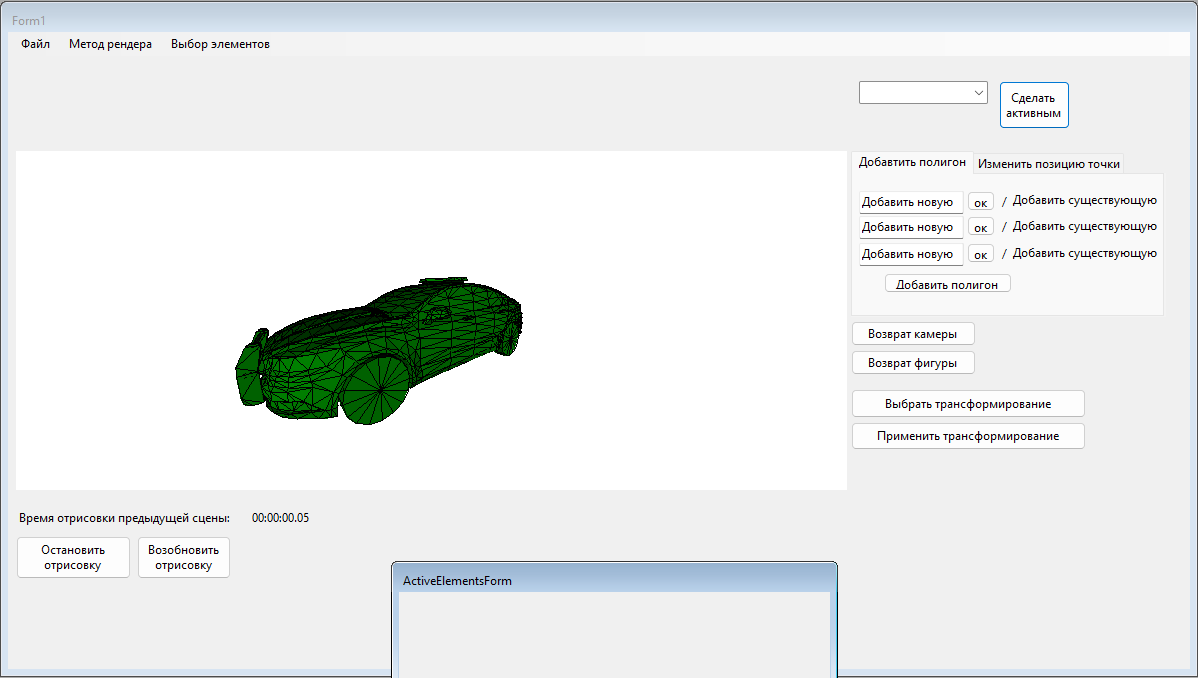
\includegraphics[ scale=0.5]{src/screen}}
	\captionof{figure}{Интерфейс программы}
	\label{img:interface}
\end{center}
\begin{center}
	\centering{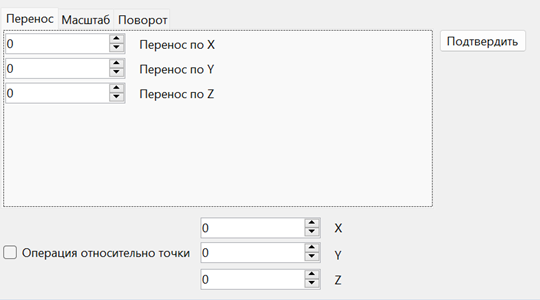
\includegraphics[ scale=1]{src/screen2}}
	\captionof{figure}{Интерфейс программы}
	\label{img:interface2}
\end{center}